\section{Automated Planning}
	\subsection{Definition of classical planning}
		Trouver une séquence d'action pour accomplir l'objectif, c'est une combinaison de différentes technique de IA:
		\begin{itemize}
			\item Seaching (Uninformed et informed)
			\item CSP
			\item Prositional logic
			\begin{itemize}
				\item Modélisation
				\item Inference (SAT)
			\end{itemize}
			\item FOL
			\begin{itemize}
				\item modelisation
			\end{itemize}
		\end{itemize}
		
		L'environnement est :
		\begin{itemize}
			\item Entierement observable
			\item déterministe 
			\item fini
			\item statique
			\item discret
		\end{itemize}
		
		C'est similaire a un \textit{Search problem} :
		\begin{itemize}
			\item Input :
			\begin{itemize}
				\item Ensemble de state
				\item Action (State $\rightarrow$ State)
				\item Initial state
				\item Goal (1 ou un ensemble de state)
			\end{itemize}
			\item Output
				\begin{itemize}
					\item Séquence d'actions
				\end{itemize}
				
			\item Difficulté : 
				\begin{itemize}
					\item Taille de l'espace de recherche
					\item Methode de recherche
					\begin{itemize}
						\item Goal test = black box
						\item doit implementer actions pour chaque probleme.
					\end{itemize}
					\item Introduire décomposition du probleme
				\end{itemize}
		\end{itemize}
		
		Son language de représentation est le PDDL (Planning Domain Definitions Language)
		
		\subsubsection{Représentation du State}
			C'est un conjonction de (Ground et function free\footnote{Ground veut dire sans variable et function free veut dire qui change en fonction du temps}) atoms ($\{A,B\} = A\land B$)
			\begin{equation}
				At(Plane1, Melbourne) \land In(Plane1, Bob)
			\end{equation}
			
			\textbf{\textit{Closes-World Assumption}} : si pas d'information sur $p(a)$ alors $p(a) = False$
			
			Dois toujours avoir des variables At(x, MEL) ne peut pas etre dans le state, pareil pour les négation $\neg$At(Plane1, MEL) ne peut pas etre dans le state, de meme on ne peut pas mettre de fonction AT(Spouse(Ali), MEL).
			
		\subsubsection{Représentation des Actions}
			Un action définis ce qui change. c'est un sous ensemble restraint de FOL.
		
			Spécifiés avec une \textbf{signature} (noms et paramètres), \textbf{Préconditions} (conjunction of literals), \textbf{Effets} (conjunction of literals)
			ex:
			
			Action(Fly(p, from, to)
			
			Precond : at(p,from) $\land$ Plane(p) $\land$ Airport(From) $\land$ Airport(to)
			
			Effect : $\neg$ At(p,from) $\land$ At(p,to) )
			
			On peut aussi utiliser comme \textbf{Ground action} sans variables 
			
			Action(Fly(P1, SFO, JFK)
			
			Precond : at(P1,SFO) \dots \footnote{tu as compris}
			
			Une action est \textbf{Applicable} dans une state $s$ si et seulement si le préconditions de $a$ est une conséquence logique de $s$ si et seulement si $s$ satisafait les préconditions de $a$
			
			Le fait que si on retire les negations est que on a pas d'information sur eux donc on les retire sur du state.
			
			\begin{figure}[H]
				\centering
				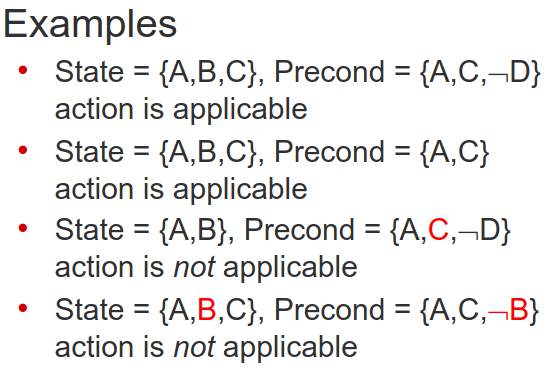
\includegraphics[width=0.5\textwidth]{img/ex.png}
			\end{figure}
			
			L'application d'une action a un state retourne un state où :
			\begin{itemize}
				\item Pour un literal A dans l'effet, il est ajouter au State
				\item Pour un litéral A négatif ($\neg A$) dans l'effet, il est retirer du state.
			\end{itemize}
			
			Ex:
			State = $\{A,B,C\}$ et Effecte = $\{E,\neg A\}$
			
			NewState = $\{B,C,E\}$, on a ajouter E et retirer A
			
			
			
			
			
		\subsubsection{Représentation des Goals}
			Une objectif = une state partiellement spécifié
			
			C'est comme une précondition : une conjonction de litérals (+ ou -)
			
			Un state satisfait un Goal si il contient tous les atoms du goals
		
			
			
			\begin{figure}[htp]	
				\centering
				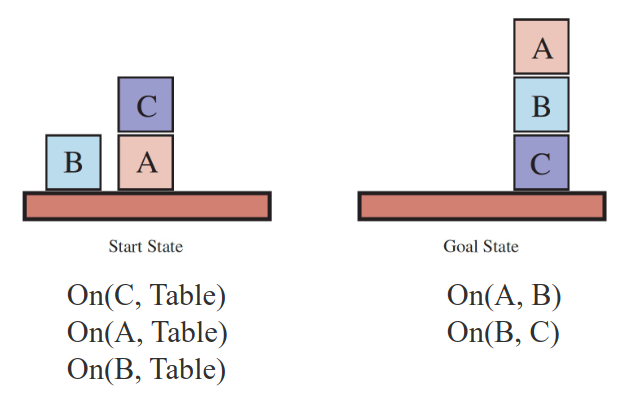
\includegraphics[width=0.8\textwidth]{img/BLOCK.png}
				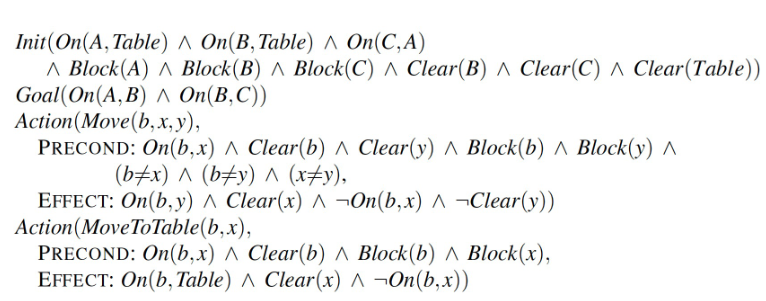
\includegraphics[width=0.8\textwidth]{img/BLOCK1.png}
			\end{figure}
			
			Voire exemple Air Cargo ou Spare tire Livre pour plus.
			 \newpage
			
	\subsection{Algorithms for classical planning}
		\subsubsection{Complexité}
			\textbf{PlanSAT} : Demande si il existe un plan qui résoud le planning probleme
			
			\textbf{Bounded PlanSAT} : Demande si il existe une solutions de longueur $k$ ou moins
			
			Les 2 problemes sont décidable (nombre fini de state)
			
			Les 2 problemes sont dans \textbf{PSPACE} (plus difficile que NP) mais pas dans NP, PlanSAT est dans P, Bounded PlanSAT est dans NP-Complet.
			
		\subsubsection{Forward and backward search}
			c'est possible d'utiliser \textit{classical state-space search methods} et avec préconditions/effetst, il es possible de rechercher dans n'importe quelle directions
			
			\begin{figure}[htp]	
				\centering
				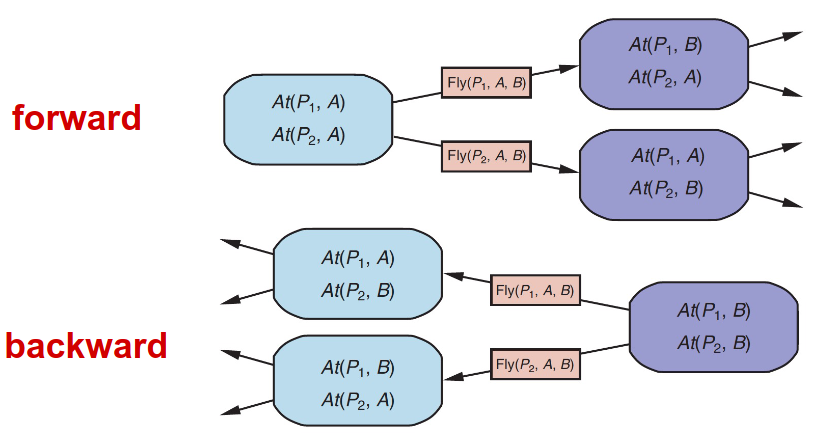
\includegraphics[width=0.8\textwidth]{img/FBSearch.png}
			\end{figure}
			
		\subsubsection{Forward state-space search}
			Similaire a la Search Methode (Ch. 3)
			
			Explore pas mal d'actions inutile, de plus state space est tres large(branching factor) c'est pour ca que une fonction heuristique précises est tres utile
			
		\subsubsection{Backward state-space Search}
			On commence du goal et on applique des actions a l'envers jusqu'a trouver une séquence d'etapes qui arrive au state initial. Marche seulement comment on sait faire une actions a l'envers pas toujours le cas. Dure de trouver un bon heuristique.
			
		\subsubsection{Planning as Boolean satisfiability}
			Planning par tester la satisfesabilité le phrase propositionnel $InitialState \land AllPossibleActionDescription \land Goal$
			
			A TERMINER
			
	\subsection{Heuristics for planning}
	
		Recherche forward ou backward est inutile sans un bon heuristique
		
		On cherche a approximer le nombre d'action pour arriver a l'objectif depuis un state donnée
		
		\subsubsection{Relaxed problem}
			On defini un nouveau probleme qui est plus facile a résoudre que le probleme initial, le cout de la solutions de ce probleme devient l'heuristique du probleme initial. On peut par exemple ignorer préconditions heuristique, 
		
		\subsubsection{Set covering Problem}
		
		On retire toutes les préconditions, et on ignonre les litérals supprimé par actions.
		
		\subsubsection{Restricted precondition}
		On retire seulement quelques literals spécifique dans les préconditions
		
		\subsubsection{Ignore-delete-list heuristic}
		Retirer la liste supprimer de toutes les actions ( supprimer l'action négatifs dans les effet )
		
		\subsubsection{Domain-independent pruning}
		Plusieurs States ne sont juste des variantes d'autre states et donc un peu inutile des les visiter et donc on va élagué certaine branche qui sont symétrique
			